% book example for classicthesis.sty
\documentclass[
  % Replace twoside with oneside if you are printing your thesis on a single side
  % of the paper, or for viewing on screen.
  %oneside,
  oneside,
  11pt, a4paper,
  footinclude=true,
  headinclude=true,
  cleardoublepage=empty
]{scrbook}

\usepackage{xcolor}
\definecolor{nicepurple}{HTML}{B10DC9}
\definecolor{niceblue}{HTML}{0074D9}
\usepackage[colorlinks=true,linkcolor=niceblue,citecolor=nicepurple]{hyperref}

\tolerance=100
\usepackage{lipsum}
\usepackage{graphicx}
\usepackage[linedheaders,parts,pdfspacing]{classicthesis}
\usepackage{acronym}
\usepackage{microtype}
\usepackage[british]{babel}

\usepackage{float}
\usepackage{caption}
\usepackage{subcaption}
\usepackage{gensymb}

\usepackage{amsmath,amsfonts,amsthm,amssymb}
\usepackage[cal=cm]{mathalfa}

\newtheorem{mydef}{Definition}
\newtheorem{myprop}{Property}
\newtheorem{mythm}{Theorem}
\newtheorem{mylem}{Lemma}
\newtheorem{mycor}{Corollary}

\graphicspath{{./Figures/}}


\title{Penrose Aperiodic Tiling of the Plane and Graphical Geodesics}
\author{Jesse Bettencourt\\1144386\\[80pt]  \textit{Supervisor: Dr. Miroslav Lovric}}

\begin{document}
\section{Ratio of Prototiles}
Recall from the substitution and Up-Down methods that we can construct tilings by decomposing Robinson triangles into smaller constituent triangles, see Fig.\ref{fig:RobSubsAgain}


\begin{figure}[H]
        \centering
        \begin{subfigure}[t]{\textwidth}
        \begin{subfigure}[t]{0.4\textwidth}
                \centering
               \raisebox{9px}{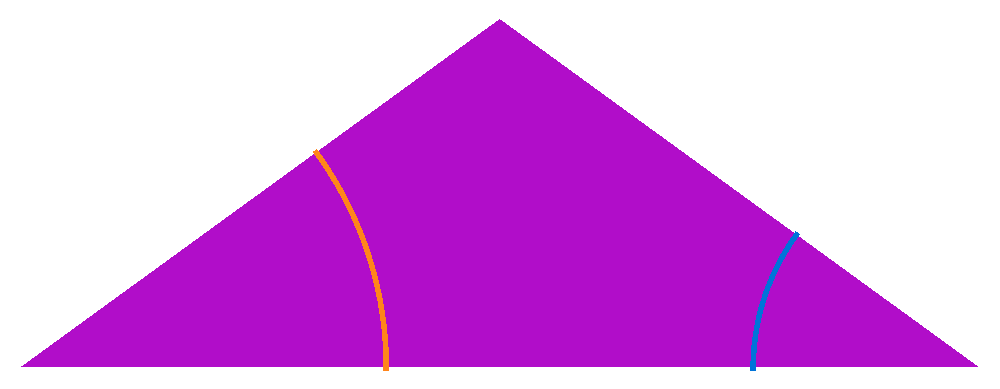
\includegraphics[scale=0.4]{RobinsonFat}}
        \end{subfigure}\hfill \raisebox{30px}{\huge$\rightarrow$} \hfill%
        ~ %add desired spacing between images, e. g. ~, \quad, \qquad, \hfill etc.
          %(or a blank line to force the subfigure onto a new line)
        \begin{subfigure}[t]{0.4\textwidth}
                \centering
                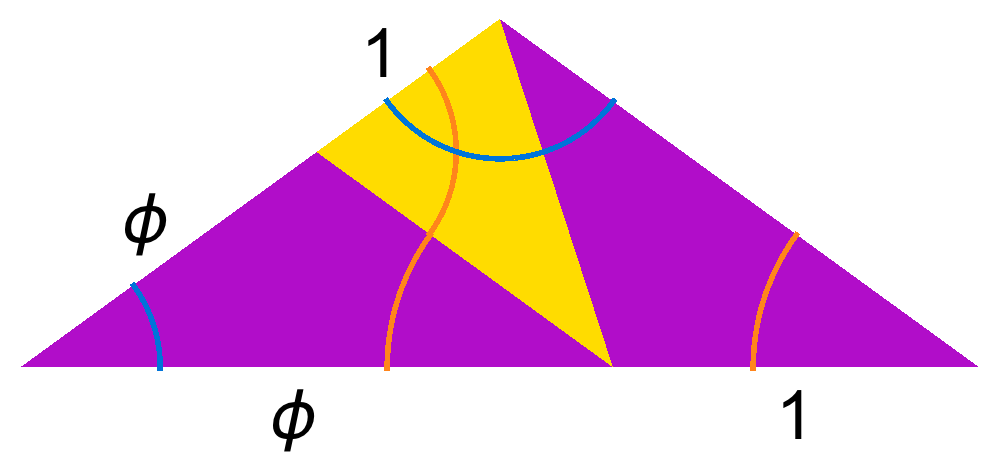
\includegraphics[scale=0.4]{RobFatSub}
        \end{subfigure}
        \caption*{$\textbf{T}=2\textbf{T}+\textbf{t}$}
        \label{fig:RobSubThickAgain}
        \end{subfigure}
        ~ %add desired spacing between images, e. g. ~, \quad, \qquad, \hfill etc.
          %(or a blank line to force the subfigure onto a new line)
          
        \begin{subfigure}[b]{\textwidth}
        \begin{subfigure}[b]{0.4\textwidth}
        \centering
		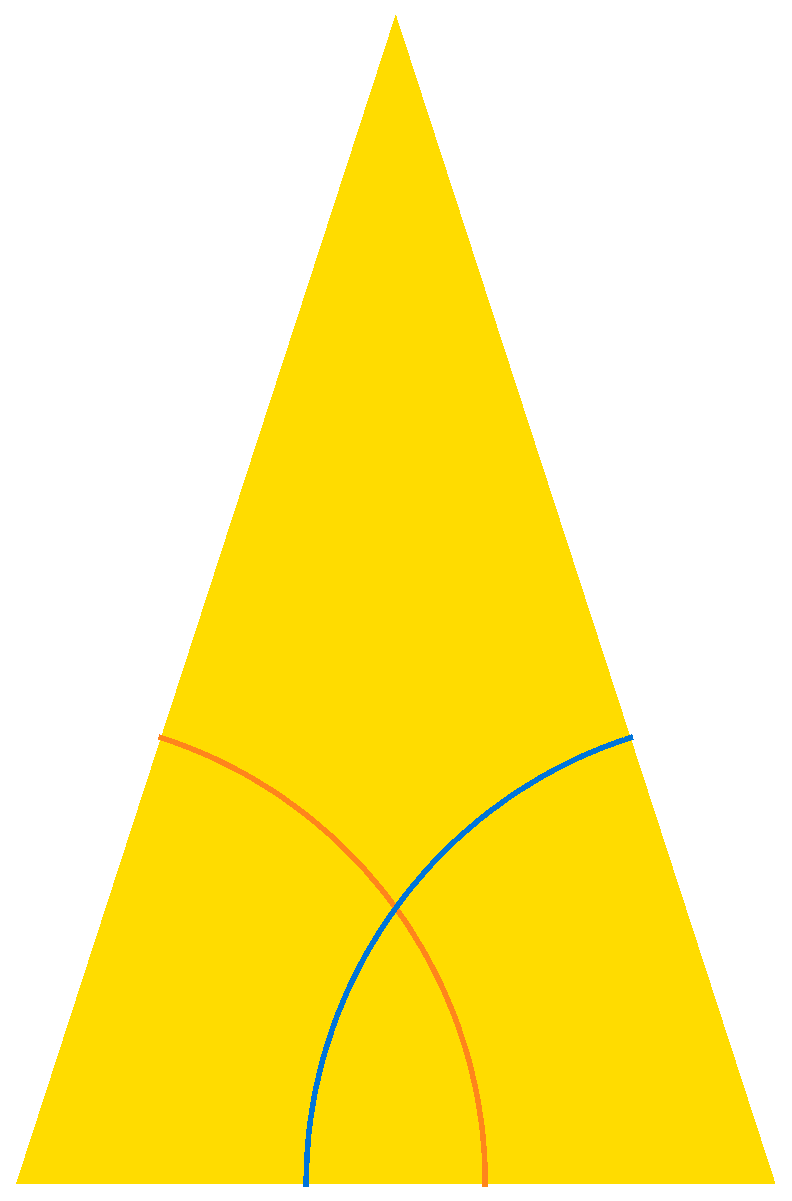
\includegraphics[scale=0.3]{RobinsonSkinny}
        \end{subfigure}\hfill \raisebox{30px}{\huge$\rightarrow$} \hfill
        \begin{subfigure}[b]{0.4\textwidth}
        \centering
                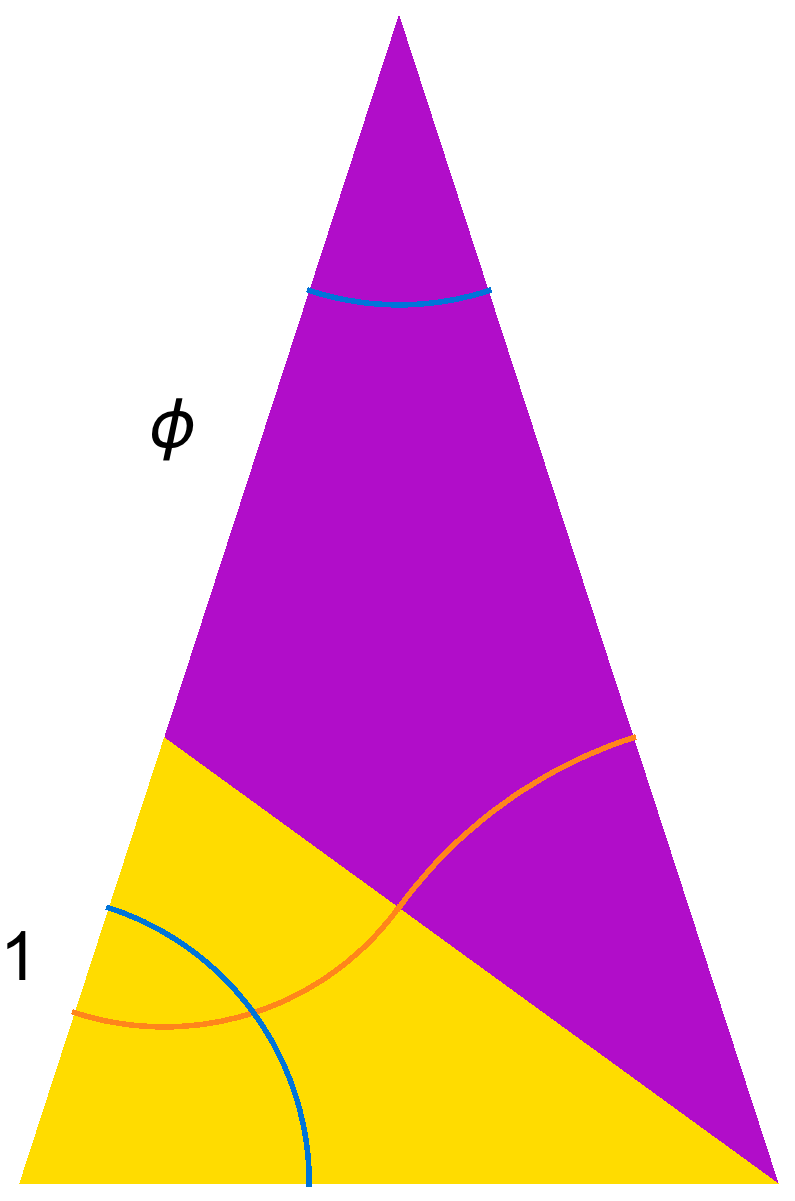
\includegraphics[scale=0.3]{RobSkinnySub}
        \end{subfigure}   
        \caption*{$\textbf{t}=\textbf{T}+\textbf{t}$}
        \label{fig:RobSubThinAgain}
        \end{subfigure}
        \caption[Robinson Triangles Deflation Again]{Decomposition equations for Robinson triangles.}
        \label{fig:RobSubsAgain}
\end{figure}

From these decomposition rules, we can define the following substitution equations for Thick \textbf{T} and Thin \textbf{t} triangles:
\begin{equation}
\begin{split}
\textbf{T}=2\textbf{T}+\textbf{t}\\
\textbf{t}=\textbf{T}+\textbf{t}
\end{split}
\end{equation}
Which can be represented by the substitution matrix:
\begin{equation}
\begin{bmatrix}
2 & 1 \\
1 & 1
\end{bmatrix}
\end{equation}
Each substitution increases the number of Thick and Thin triangles by according to this linear equation: 
\begin{equation}
\begin{bmatrix}
\textbf{T}_{i+1} \\
\textbf{t}_{i+1}
\end{bmatrix}=
\begin{bmatrix}
2 & 1 \\
1 & 1
\end{bmatrix}
\begin{bmatrix}
\textbf{T}_{i} \\
\textbf{t}_{i}
\end{bmatrix}
\end{equation}
Where $\textbf{T}_{i}$ is the number of Thick triangles prior to decomposition, and $\textbf{T}_{i+1}$ is the number after decomposition. Applying this decomposition $n$ times will give us the following:
\begin{equation}
\begin{bmatrix}
\textbf{T}_{i+1} \\
\textbf{t}_{i+1}
\end{bmatrix}=
\begin{bmatrix}
2 & 1 \\
1 & 1
\end{bmatrix}^n
\begin{bmatrix}
\textbf{T}_{i} \\
\textbf{t}_{i}
\end{bmatrix}
\label{eq:subeq}
\end{equation}
To determine the ratio of Thick triangles to Thin triangles in an arbitrarily large Penrose tiling, we consider the limiting behaviour of this equation as $n\rightarrow\infty$. One way to accomplish this is to recognize that the $n^{\text{th}}$ power of the substitution matrix has the form:
\begin{equation}
\begin{bmatrix}
2 & 1 \\
1 & 1
\end{bmatrix}^n= 
\begin{bmatrix}
F_{2n+1} & F_{2n} \\
F_{2n} & F_{2n-1}
\end{bmatrix}
\end{equation}
Where $F_n$ is the $n^{\text{th}}$ Fibonacci number.\\
Alternatively, we can describe the limiting behaviour of the $n^{\text{th}}$ power of the substitution matrices by considering its eigenvectors. The characteristic polynomial of the substitution matrix is:
\begin{equation}
\lambda^2-3\lambda+1
\end{equation}
With eigenvalues
\begin{align}
\lambda_1=\phi^2 &\quad
&\lambda_2=\frac{1}{\phi^2}
\end{align}
The eigenvectors of these eigenvalues are:
\begin{align}
v_1= \begin{bmatrix}
\phi \\
1
\end{bmatrix}
&\quad&
v_2= \begin{bmatrix}
1 \\
-\phi
\end{bmatrix}
\end{align}
These eigenvectors are orthogonal, and each with positive eigenvalue, and are unstable equilibria, Therefore, we see that the limiting behaviour the linear equation in Eq.\ref{eq:subeq} cause all initial conditions to attract to approach one of these eigenvectors away from the origin. Likewise, it is a well know fact that the ratio between two consecutive numbers in the Fibonacci sequence is $\phi$. Therefore, we see that the ratio of Thick to Thin triangles, and therefore Rhombs, is $\phi$.

One might have initially anticipated that there would be more Thin Rhombs than Thick, perhaps because we can envision Thin Rhombs filling in smaller gaps. However, we see that this is not the case.

More surprisingly, however, is that this ratio is irrational. This provides deep insight into the aperiodicity of the tiling. If the tiling was periodic, then the global ratio of the tiles will be the same as the ratio of the infinitely repeating subregion which defines the periodic tiling. However, since we know that aperiodic tilings cannot be represented by a single, infinitely repeating region, this is not insightful for aperiodic tilings. The irrationality of the tiling ratio informs us that aperiodic tilings exist at the infinite limits of these processes. Of course, the number of Thick and Thin tiles are both whole numbers, so how then could we ever achieve a tiling where their ratio is the irrational $\phi$? Only by considering the infinite limit of the tiling methods.

\bibliographystyle{unsrt}
\bibliography{bibliography}    
\end{document}